\subsection{\labeltext[Diagrama de Atividades - Funcionário]{Diagrama de Atividades - Funcionário}{er:241}}

\begin{figure}[H]
	\centering
	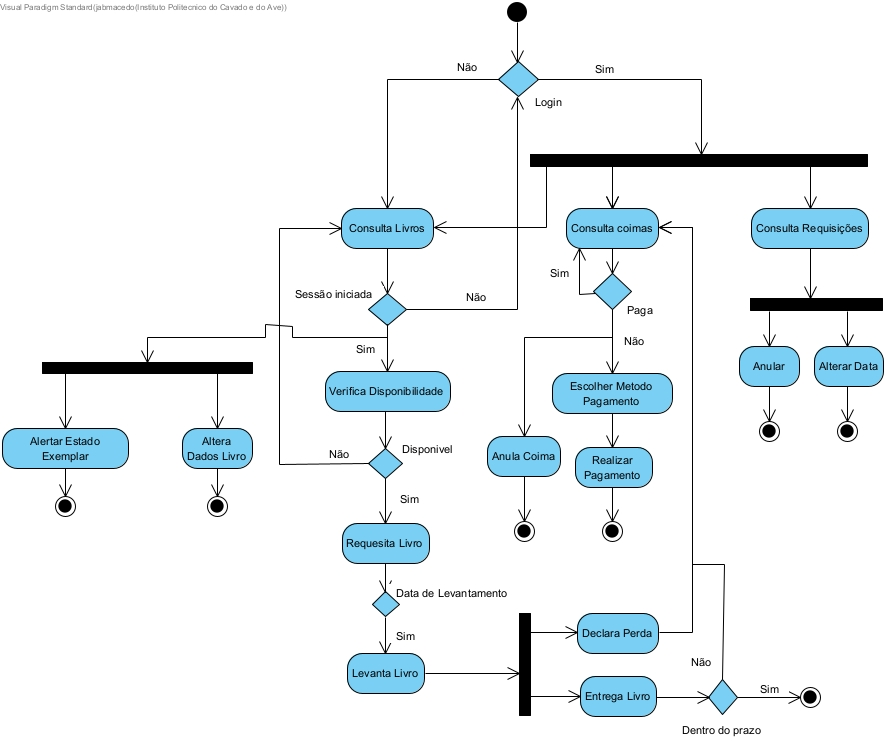
\includegraphics[width=1\linewidth]{./img/Diagramas_A/DA_Funcionario.jpg}  % largura percentual 
	\caption{\ref{er:241}}
	\label{fig:chap241}
\end{figure}

Com base no diagrama de atividade do funcionário, presente acima, é possivel observar que o mesmo possui um esquema identico ao do utilizador com apenas algumas adições e ligeiras alterações.
Um bom exemplo de uma alteração é quando observamos a consulta de requisições, já não sendo necessário o prazo de até 24h.
Quanto a funcionalidades adicionais, as principais são relativas aos exemplares/livros, o funcionario pode alertar o admin quanto ao estado de um determinado exemplar para que o admin possa proceder quanto ao tratamento dessa informação da melhor forma, e pode também alterar certos dados do livro, como o titulo, descrição, entre outros.